%from arXiv:1212.5127v2
\section{DECAL}
Most recent update: 2014-08-25 \\
Contact person: Jan Strube (email: jan.strube@pnnl.gov)

\subsection{Introduction}
The studies of a digital ECAL (DECAL) in the UK are currently dormant. In December 2008, the STFC Executive recommended sufficient funding
to allow the SPiDER Collaboration to construct a full physics prototype DECAL, as outlined
in~\cite{Adloff:2010aa}. By December 2009, the funding for SPiDER had still not been issued and STFC
informed the Collaboration that they would not do so.

The UK groups in SPiDER have demonstrated that the INMAPS technology developed
specifically for the DECAL application is viable in terms of basic pixel efficiency. INMAPS is
implemented as a \SI{0.18}{\micro\meter} CMOS process in which a deep P-well implant stops signal charge
from being absorbed in N-well circuits, and therefore allows the use of both NMOS and
PMOS within the pixel, as well as (optionally) high resistivity silicon in the thin epitaxial
layer to reduce the charge collection time.

\subsection{Test Beams in 2010}
Following a successful test beam run at CERN in September 2009 using 120 GeV pions, two
further data taking runs have been carried out. The first of these was at DESY in March
2010, for which the primary goal was to quantify the peak electromagnetic shower density
observed downstream of specific absorber materials. A secondary goal was to make further
pixel efficiency measurements. Data were recorded with the 1-5 GeV electron beam, using a
configuration in which four TPAC 1.2 sensors were aligned precisely along the beam direction
using the same custom-built mechanical frame as at CERN. Absorber material (W, Fe, Cu)
was placed downstream of these, followed immediately by a further pair of TPAC sensors, to
study the shower density.

To complement the DESY run, similar, additional data was recorded at CERN in September 2010, using the EUDET telescope alone as it has finer pitch than the TPAC sensor, with positrons between 10 and 100 GeV. The same slabs as those at DESY were used together with
new slabs due to the higher energies available at CERN. Initial results of shower multiplicities
are presented in~\cite{Price:2012vta}.

\subsection{Pixel efficiency results}
The studies of pixel efficiency from CERN 2009 testbeam and DESY were performed using a
set of six TPAC 1.2 sensors aligned along the beam direction, in which the outer four sensors
served as a beam telescope, while the two innermost sensors were considered as the devices
under test. The trajectory of the beam particle was projected onto the plane of both of these
sensors, and each pixel of the test sensors was examined for the presence of hits as a function
of the distance from the projected track. The MIP hit efficiency was determined by fitting
the distribution of hit probability to a flat top function, convoluted with a Gaussian of the
appropriate resolution to allow for finite tracking performance. This efficiency, folded for all
pixels together, is illustrated in Figure~\ref{fig:Calorimeter:DECAL:MIPS}

\begin{figure}
    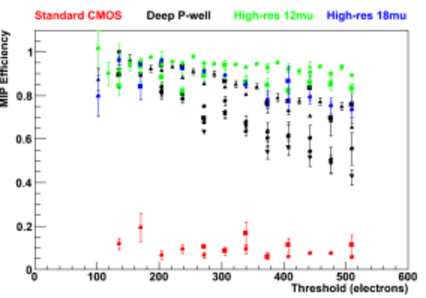
\includegraphics[width=.49\textwidth]{Calorimeter/DECAL/MIPEfficiency}
    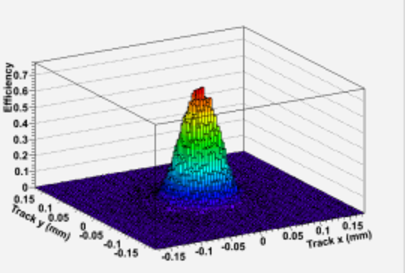
\includegraphics[width=.49\textwidth]{Calorimeter/DECAL/MIPResponse}
    \caption{(left) Distribution of the probability of a pixel registering a hit in response to a MIP, as a function of distance to the projected track, and (right) MIP efficiency as a function of the sensor digital threshold, for all four sensor variants studied.}
    \label{fig:Calorimeter:DECAL:MIPS}
\end{figure}

The MIP efficiency was determined per pixel for both the DESY and CERN data, and for each of the four pixel variants tested. The variants (and corresponding marker color in Figure~\ref{fig:Calorimeter:DECAL:MIPS}) are:

\begin{enumerate}
\item (red) in \SI{12}{\micro\meter} standard (non-INMAPS) CMOS;
\item (black) \SI{12}{\micro\meter} deep P-well CMOS;
\item (green) deep P-well within a \SI{12}{\micro\meter} high resistivity epitaxial layer;
\item (blue) deep P-well within an \SI{18}{\micro\meter} high resistivity epitaxial layer.
\end{enumerate}

The results~\cite{Dauncey:2010zz} are summarized in Figure~\ref{fig:Calorimeter:DECAL:MIPS}, for a range of the sensor digital thresholds representative of the signal levels expected in DECAL pixels due to charge spreading. (A typical MIP signal in a \SI{12}{\micro\meter} epitaxial layer of silicon is 1200 electrons and a single pixel absorbs at most 50\% of this due to charge spreading.)

From the results shown in the figure, it is observed that the standard, non-INMAPS sensors have markedly low efficiencies, which is attributed to signal charge being absorbed by in-pixel PMOS transistors. In contrast, the use of the deep P-well reduces the absorption of signal charge by N-wells in the circuitry, improving very substantially the pixel efficiency by a factor of $\approx 5$. The addition of the high resistivity epitaxial layer further improves the pixel efficiency to $\approx 100\%$.

\subsection{Future plans}
It is no longer an option to plan for a physics prototype DECAL and the short-term future of the DECAL project is extremely uncertain at present. A program of radiation hardness has been conducted on 2011 and the results are summarized in~\cite{Price:2012vta,Price:2013js}. This is in part to understand how the TPAC sensor would satisfy the requirements of ALICE ITS and SuperB . The studies which have been carried out so far are in the process of being finalized, and a series of papers, e.g.~\cite{Ballin:2011jq}, are in preparation to document what has been achieved. The technology development has been taken over by the Arachnid collaboration who are testing the CHERWELL chip (designed and manufactured by the SPiDeR collaboration but never used due to money constraints) to evaluate the performance for ALICE and SuperB.
